\section{Experimentelles Vorgehen}
\begin{figure}[]
  \centering
  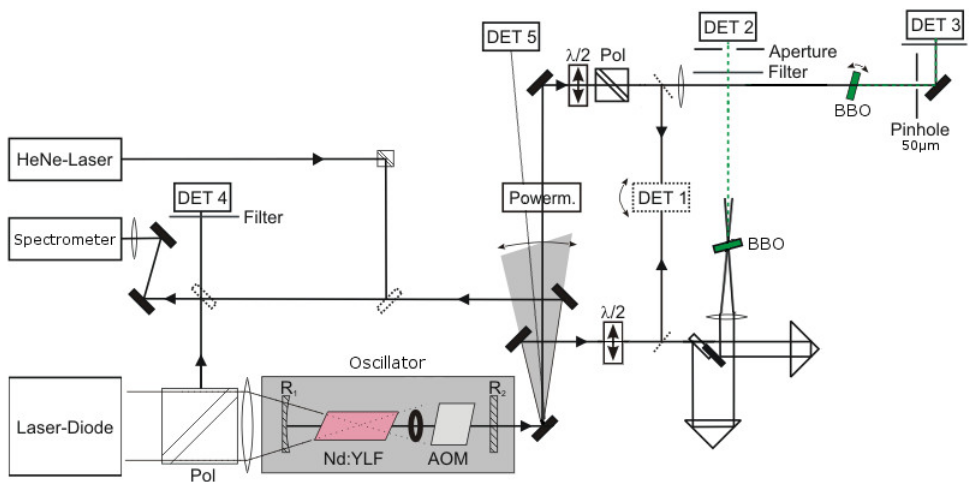
\includegraphics[width = 0.8\textwidth]{Bilder/Versuchsaufbau.png}
  \caption{Schematischer Versuchaufbau}
  \label{fig:versuchsaufbau}
\end{figure}
Die Versuchsanordung für das Laserexperiment ist in Abbildung \ref{fig:versuchsaufbau}
zu sehen. Als Erstes wurde die Leistungs-Kennlinie der Pumplaserdiode aufgenommen, um deren Wirkungsgrad festzustellen.
Als Nächstes wurden durch vorsichtige Verstellung der Resonatorlänge die Moden der einzelnen Laser betrachtet.
Für die nächsten Versuche wurde die gaußförmige Mode gewählt, da sich diese am besten für
die Erzeugung von Ultrakurzpulsen eignet.
Mit dieser Einstellung und den Angaben der Pumplaserdiode wurde der
Wirkungsgrad des Nd:YLF Lasers bestimmt. 
Danach wurde der akustooptische Modulator für die Erzeugung der Ultrakurzpulse angeschaltet, und mithilfe des Signals einer Halbleiterdiode die Resonatorlänge so eingestellt dass der Pulspeak maximal war.
Mithilfe der Verzögerungsstrecke und einem optischen Kristall wurde das Autokorellationssignal des Pulses gemessen.
Mit einem Präzisionsdrehtisch wurden dann die Eigenschaften des $\beta$-Bariumoxid-Kristalls untersucht, um festzustellen, bei welchem Orientierungswinkel der Kristall am effizientesten die zweite Harmonische, also grünes Licht generiert.
Danach wurde über die Rotation eines $\frac{\lambda}{2}$-Plättchens die Intensität des auf den optischen Kristall einfallenden Lichtes reguliert, um den Zusammenhang zwischen Intensität des einfallenden Lichtes und der Oberwelle zu messen.
Zuletzt wurden mithilfe eines Spektrometers die Spektren der Pumpdiode bei drei verschiedenen Stromstärken bestimmt. Dabei konnte man genau die Übergänge zwischen spontaner Emission, beginnener Laseraktivität und Laseraktivität deutlich erkennen. Als letztes wurde das Laserspektrum des Nd:YLF Lasers, welches für spätere Berechnungen benötigt wird.

%%% Local Variables:
%%% mode: latex
%%% TeX-master: "../Laser"
%%% End:
